\chapter{Optimization}

The solution presented in Chapter~\ref{chap:solution}, despite
providing correctness guarantees and ease of use, performs poorly even
in trivial test cases. This chapter describes a series of
optimizations made to keep the overhead as low as possible, without
sacrificing correctness.

\section{Example Application}

To perform accurate measurements, I developed a sample banking
application. In this application's domain (see
Listing~\ref{list:bank-dml}) there is a central Bank with Customers,
which in turn have their accounts. For each account the application
keeps its balance, and there is a method to show a
customer's balance (by summing the balance of all his accounts). Every
time a transaction is done, a new TransactionRecord is created,
containing a timestamp, the origin and destination accounts, as well
as the amount transfered.

\begin{lstlisting}[caption={Domain Model for the Banking Application},
  label={list:bank-dml},float]
class Bank;
class Customer;

class Account {
  Double balance;
  DateTime opened;
}

class TransactionRecord {
  DateTime when;
  Double amount;
}

relation BankHasCustomers {
  Customer playsRole customer {
    multiplicity *;
  }
  Bank playsRole bank;
}

relation CustomerHasAccounts {
  Customer playsRole owner {
    multiplicity *;
  }
  Account playsRole account {
    multiplicity *;
  }
}

relation TransactionRecordHasFrom {
  Account playsRole from;
  TransactionRecord playsRole outgoingTransaction {
    multiplicity *;
  }
}

relation TransactionRecordHasTo {
  Account playsRole to;
  TransactionRecord playsRole incomingTransaction {
    multiplicity *;
  }
}
\end{lstlisting}

In this scenario, a Business Transaction will consist of several
banking transactions, spread throughout a series of Business
Operations. This is the perfect candidate for a Long Lived
Transaction.

In the {\it regular} scenario, each business operation will run within
a regular JVSTM transaction (and thus every intermediate state is
visible to the outside world), whereas in the {\it Long Lived}
scenario the Business Transaction is mapped into a Long Lived
Transaction, and each individual operation runs within an LLT step
(meaning that intermediate state will not be visible to the outside).

With the support presented in previous sections, the programmer simply
writes the application's code as he would without considering Long
Lived Transactions. No changes to the data structures and business
logic are required. Listing~\ref{lst:invoc-diff} shows the two methods
used to invoke both versions under test. Notice that they both look
very similar as they both invoke the \texttt{doScript} method, the
only difference is that in the LLT version, a new
\texttt{TransactionalContext} is created and bound to the current
thread.

\begin{lstlisting}[caption={Invoking the business operation},
 label={lst:invoc-diff},float]
public void doRegular() {
  doScript("regular");
}

public void doLongTx() {
  TransactionalContext context = createContext();
  LongTransaction.setContextForThread(context);
  doScript("long");
  LongTransaction.removeContextFromThread();
}
\end{lstlisting}

Using this banking domain, a sample application was developed. In this
fictitious scenario, the bank starts with a certain number of
customers (this number is configurable so that different parameters
may be measured), and creates a Long Lived Transaction with a
configurable number of operations. Within each operation, new
customers and accounts are created, money is be shuffled between all
the bank's accounts (creating a new TransactionRecord for each
transaction), and the total balance is calculated. This means that in
each step: (1) Every object in the system is read, (2) Many objects
are written and (3) Many new objects are created.

\begin{lstlisting}[caption={Code for the Business Operation},
float]
// Bank class
public double getTotalMoney() {
  double money = 0;
  for (Customer customer : getCustomerSet())
    money += customer.getTotalMoney();
  return money;
}

// Customer class
public double getTotalMoney() {
  double money = 0;
  for (Account account : getAccountSet())
    money += account.getBalance();
  return money;
}

public void shuffle() {
  Account firstAccount = getRandomAccount();
  for (Account account : getAccountSet()) {
    if (!firstAccount.equals(account)) {
      account.transfer(account.getBalance(), firstAccount);
    }
  }
}

// Account class
public void transfer(Double amount, Account to) {
  this.withdraw(amount);
  to.deposit(amount);
  addOutgoingTransaction(new TransactionRecord(to, amount));
}

// Benchmark class
@Atomic(mode = TxMode.WRITE)
public void doOperation() {
  createCustomers();
  logger.info("Bank has {} money.", bank.getTotalMoney());
  shuffleMoney();
  shuffleMoney();
  logger.info("Bank has {} money.", bank.getTotalMoney());
  createCustomers();
  shuffleMoney();
  logger.info("Bank has {} money.", bank.getTotalMoney());
}

private void createCustomers() {
  for (int i = 0; i < ACCOUNTS; i++) {
    Customer customer = new Customer("Customer " + counter++);
    customer.addAccount(new Account(200d));
    customer.addAccount(new Account(100d));
  }
}

private void shuffleMoney() {
  for (Customer customer : bank.getCustomerSet())
    customer.shuffle();
}
\end{lstlisting}


\section{Initial Performance Analysis}

Figure~\ref{fig:regTime} shows the running time for a varying number
of operations of the application presented above. As expected, the
running time grows linearly as the number of operations increases.

When looking at the Long Lived version (where every operation is a
step of a large Long Lived Transaction), performance quickly degrades
as the number of operations grows. The main reason for this
performance hit is that every box read will cause many other boxes to
be read (instead of just reading the box directly, all LogEntries
representing the write set must be traversed, meaning that many more
boxes are read along the way, and many more boxes will be read as the
transaction grows in size). Recall from Chapter~\ref{chap:ff} that in
the JVSTM using a multi-box layout, each slot of an object is kept in
a separate box, and as such reading a single Log Entry will cause at
least 3 boxes to be read: the slot name, the target object, and the
next box in the list.

Figure~\ref{fig:reg-box} shows that in a regular transaction, the
number of boxes read grows slowly as with the number of
operations. The same behaviour is observed with Long Lived
Transactions: Figure~\ref{fig:long-box-v1} shows that the number of
boxes read grows following the same pattern as the running time.

As reading boxes is one of the major sources of the poor performance
results of this implementation, I made several improvements regarding
the number of boxes read and boxes written. The next sections present
those optimizations.

\begin{figure}
\centering
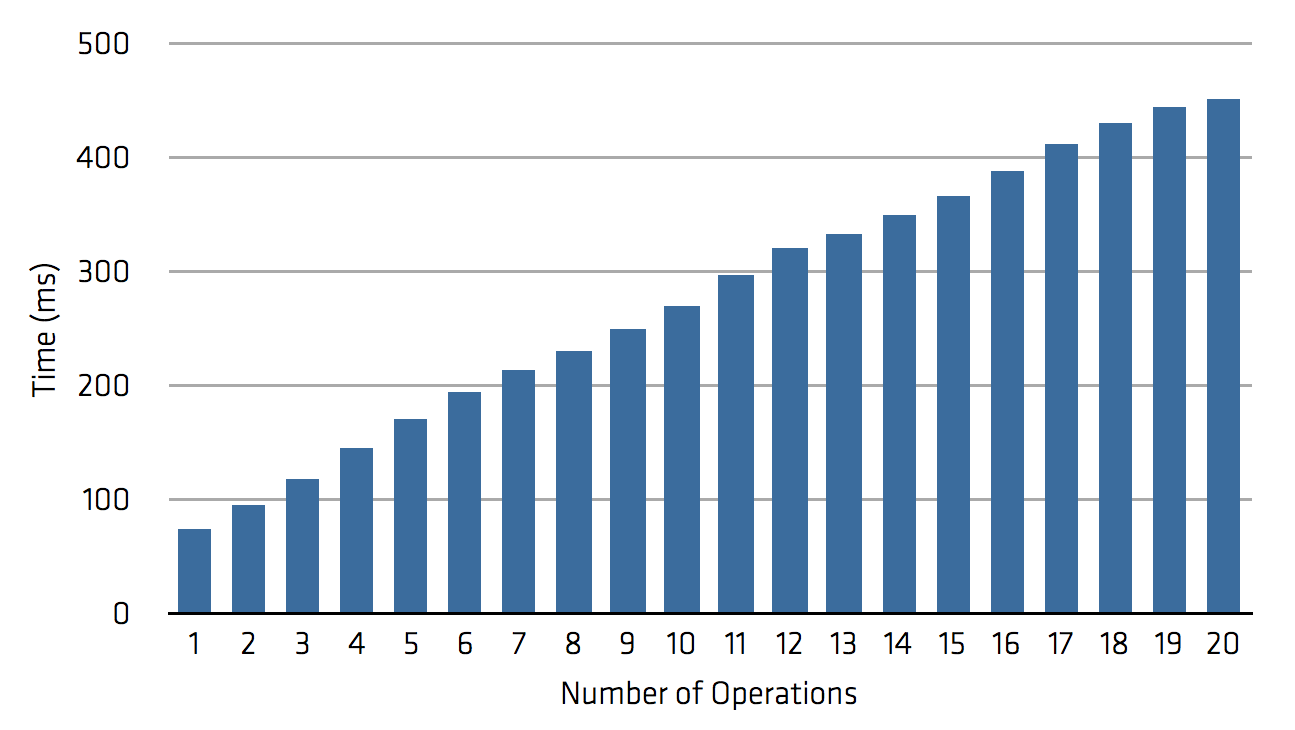
\includegraphics[width=0.9\linewidth]{time-regular}
\caption{Running time with regular transactions}
\label{fig:regTime}
\end{figure}

\begin{figure}
\centering
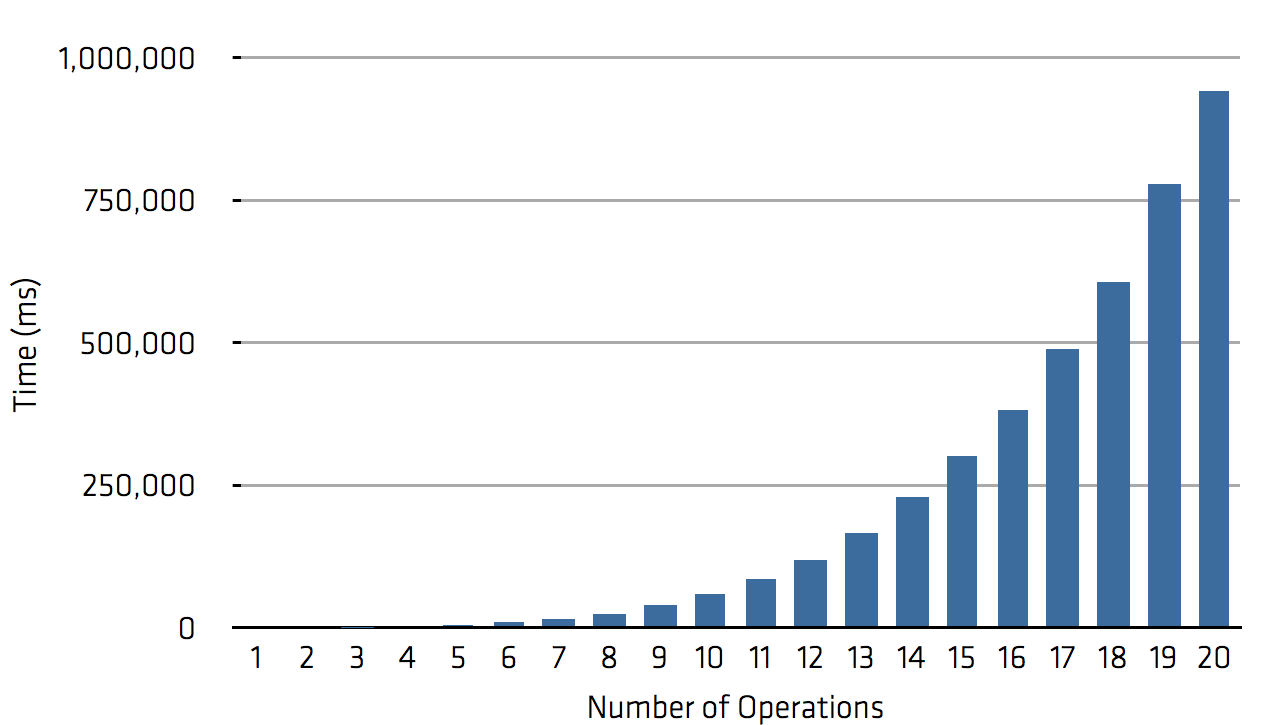
\includegraphics[width=0.9\linewidth]{time-long-v1}
\caption{Running time with Long Lived Transaction steps}
\end{figure}

\begin{figure}
\centering
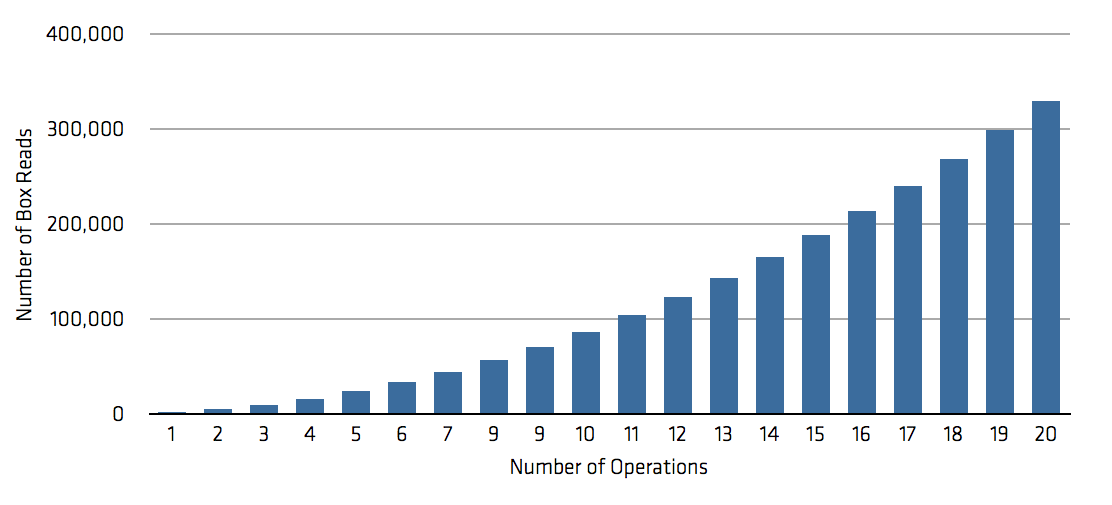
\includegraphics[width=0.9\linewidth]{box-regular}
\caption{Number of boxes read on a regular transaction}
\label{fig:reg-box}
\end{figure}

\begin{figure}
\centering
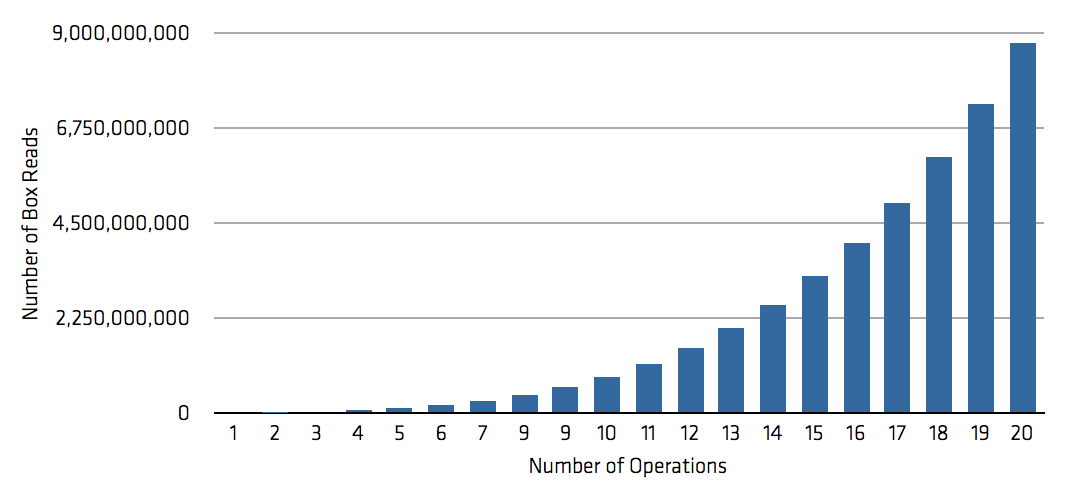
\includegraphics[width=0.9\linewidth]{box-long-v1}
\caption{Number of boxes read using Long Lived Transaction steps}
\label{fig:long-box-v1}
\end{figure}

\section{Read-Set differentiation}

In the initial implementation, {\it LogEntries} were used to reify
both the Read Set and the Write Set.

Recalling Figure \ref{fig:transactionalContext}, {\it LogEntries} store a
reference to the DomainObject they refer to, the name of the slot, and
the slot's value. Using the same objects to represent both sets proved
to be quite expensive, as the Read Set only cares about which slots
were read, completely ignoring its value.

By analysing the nature of the Read Set, we may conclude that it is
only necessary to store the pairs [DomainObject, Slot] read by the
transaction (the actual version read is not relevant, as it will
always be coherent with the transaction's version).

As such, the Read Set has been replaced by an immutable
ValueType\footnote{ValueTypes are explained in detail in Chapter
  \ref{chap:ff}.}, containing a set of DomainSlotKey's (an immutable,
lightweight object representing the pair [DomainObject, Slot]), stored
directly into the {\it TransactionalContext}.

This optimization greatly reduced the space required by the
Transaction (both in-memory and persistently), as the representation
of the Read-Set became more compact (a single slot in an object vs
several objects).

The commit time for the various steps of the Transaction also
improved, as the lookups/insertions of entries in the Read Set are
done entirely in memory, without the need to traverse (and
potentially reload a large object graph).

\section{Using BPlusTrees to hold LogEntries}

As described in Chapter \ref{chap:ff}, the Fenix Framework uses
BPlusTrees and other collections to implement to-many relations. These
collections are transparently handled by the Framework, and are
implemented using regular Domain Objects (such as Leaf Nodes and Inner
Nodes). As keeping track of changes in relations is a requirement for
our implementation, it is critical that changes to BPlusTrees are
correctly tracked.

This posed a great issue, as conceptually one
\texttt{TransactionalContext} has many \texttt{LogEntries} in both its
Read and Write Sets. If this relation were to be implemented using a
regular one-to-many relation, a BPlusTree would be generated by the
Framework. But as BPlusTrees must be tracked by the
\texttt{TransactionalContext}, they could not be used to implement
this relation.

The initial approach to this problem consisted on implementing the
relation using a Linked List, in which a LogEntry would be directly
connected to the next one in the list, keeping the list sorted by
insertion order. Figure~\ref{fig:linkedList} shows how this was
designed. This approach proved to be quite inefficient, as lookups in
the Write Set were {\it O(n)} in the number of written objects, making
it impractical, as every \texttt{getBoxValue} operation required
potentially traversing the whole list.

\begin{figure}
\centering
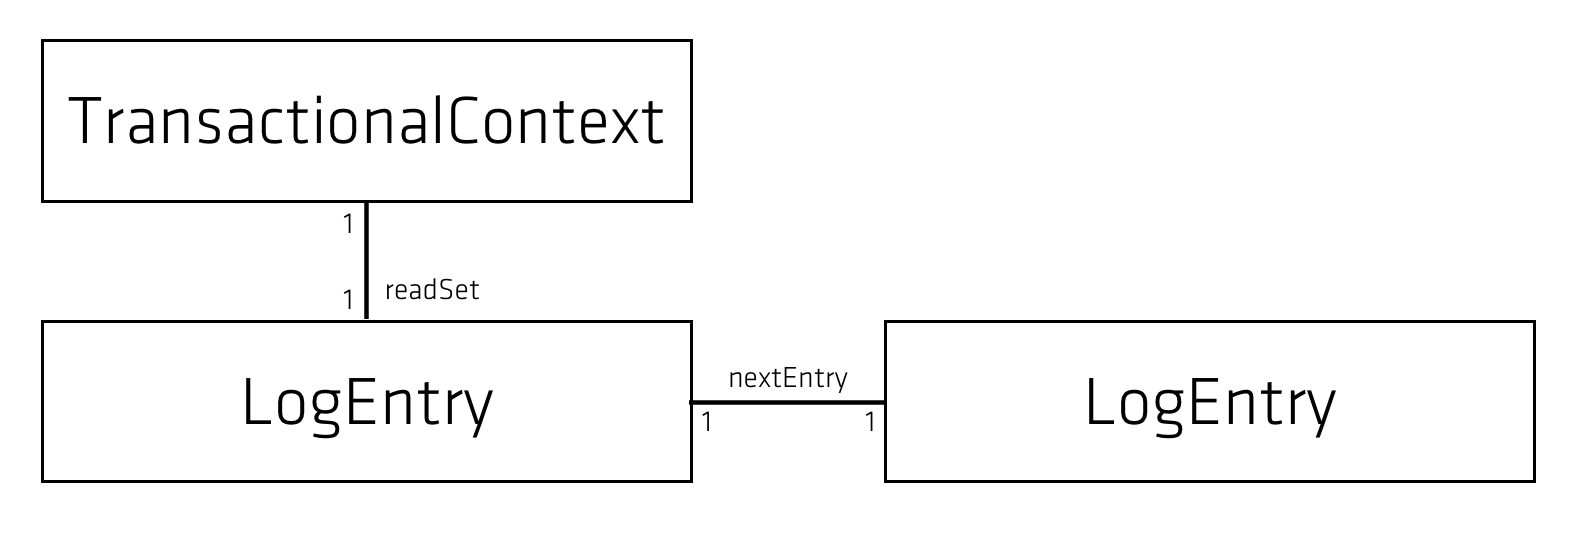
\includegraphics[width=0.7\linewidth]{tx-context-v1}
\caption{LogEntry linked lists}
\label{fig:linkedList}
\end{figure}

To solve this issue, a specialised \texttt{WriteSetBPlusTree} was
developed. The major difference between a \texttt{WriteSetBPlusTree}
and a regular BPlusTree is that the former is designed to be kept out
of the scope of the TransactionalContext, making it possible to use it
to implement the one-to-many relation between a TransactionalContext
and its LogEntries.

Another advantage of directly using a BPlusTree is that it is possible
to take full advantage of all its features. Generically speaking, a
BPlusTree is a map between keys and values. When the Fenix Framework
generates a BPlusTree to represent a to-many relation, the map
contains the pointed objects as values, and the object's identifiers
(OID) as keys. In this case however, lookups are not performed by OID,
but by DomainSlotKey (DomainObject+slot). As such, a WriteSetBPlusTree
will map DomainSlotKeys to their corresponding LogEntries.

With this approach, looking up a DomainSlotKey in a
TransactionalContext means that the BPlusTree is indexed using the
DomainSlotKey, and as such, lookup times are now {\it O(log(n))}.

In Figures~\ref{fig:runtimeBPlus} and \ref{fig:comparisonBPlus} we can
see that the running time using BPlusTrees is now similar to the
regular version. However, the growth rate (while linear) is still
bigger than the original, with an average 4.4x performance loss. One
of the big contributors for this speed improvement seems to be the
number of Box Reads that happens throughout the transaction. Whereas
in the original implementation this number reached over 1.5B, it is
now reduced to about 3.1M.

\begin{figure}
\centering
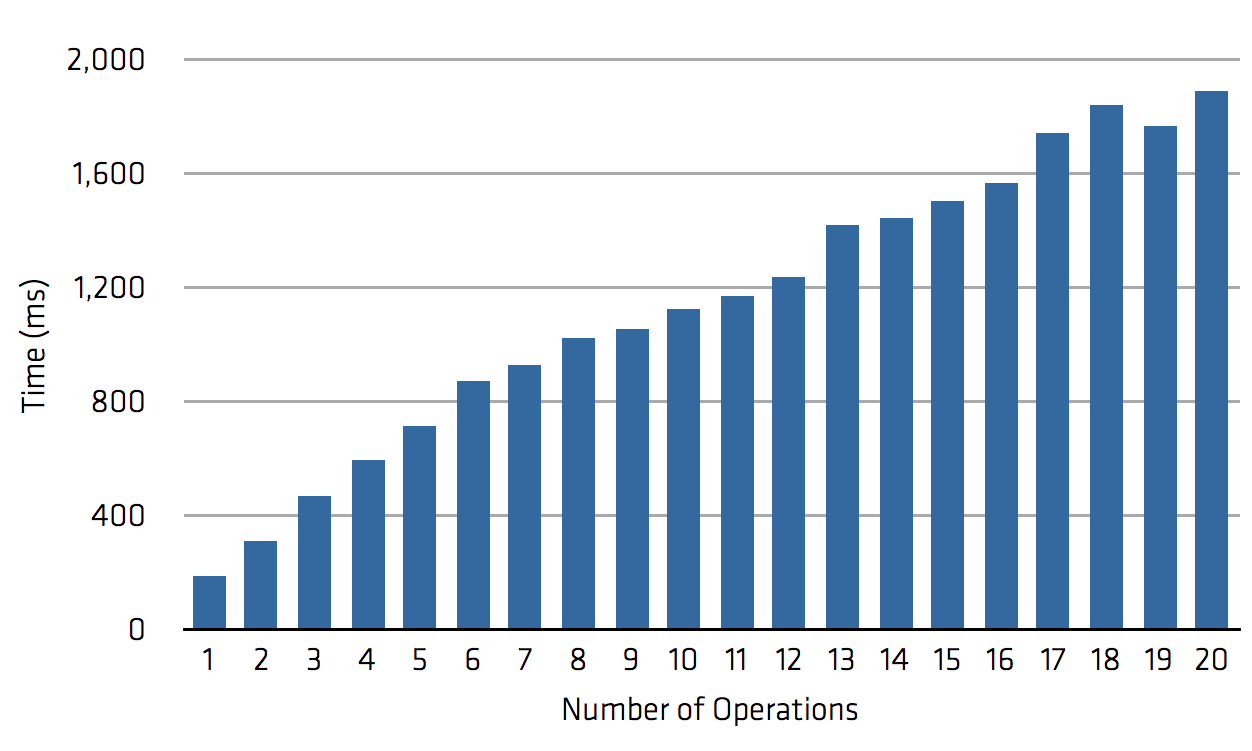
\includegraphics[width=0.9\linewidth]{time-long-bplus}
\caption{Running time using BPlusTrees}
\label{fig:runtimeBPlus}
\end{figure}

\begin{figure}
\centering
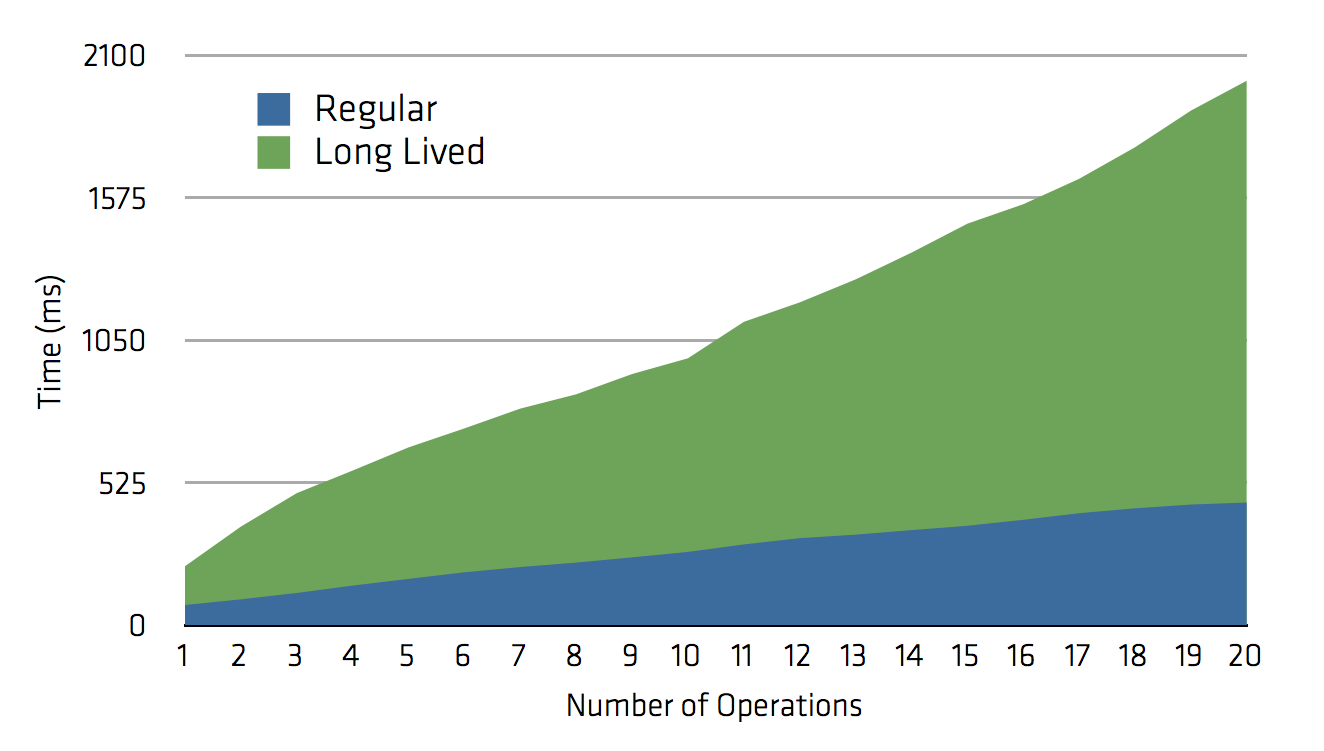
\includegraphics[width=0.9\linewidth]{comparison-bplus}
\caption{Running time comparison using BPlusTrees}
\label{fig:comparisonBPlus}
\end{figure}

\begin{figure}
\centering
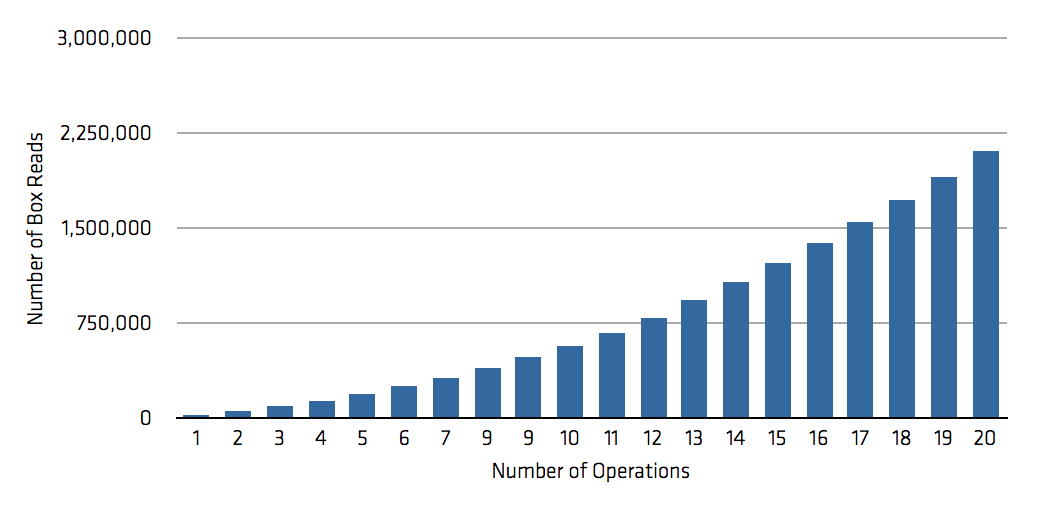
\includegraphics[width=0.9\linewidth]{box-long-bplus}
\caption{Box reads using BPlusTrees}
\label{fig:boxesBPlus}
\end{figure}


\section{Removing LogEntries}

With the relation between the {\it TransactionalContext} and the {\it
  LogEntries} implemented using a BPlusTree, another issue arisen. 

Despite having great lookup times, the commit of a Long Transactions's
step was greatly affected. Whereas inserting elements in a Linked List
is {\it O(1)}, the insertion in the BPlusTree was still painfully
slow.

This is because the Fenix Framework requires that ValueTypes (such as
the ones used to back the BPlusTree) are immutable combined with the
fact that the BPlusTree provides no API for batch insertion, meaning
that for each of the elements written within a given step, a new
insert was performed, and the backing TreeMaps were duplicated over
and over. 

The approach to solve this issue, was to use a solution similar to the
one used for the Read-Set: create an immutable ValueType, containing
the mapping between all written slots and their respective values.

With this change, {\it LogEntries} were completely taken out of the
picture, as the only extra piece of information they provided was the
JSON contents of the slot, which could be embedded directly into the
WriteSet object.

The issue with this approach is that, due to the immutability
requirement, every time a batch of entries was inserted, the whole Map
had to be duplicated, which was rather wasteful both in terms of time
and allocated memory. So, instead of duplicating the whole Map, the
WriteSet is actually a Linked-List of Maps, containing one node per
transaction step. This means that the performance of lookups is now
{\it O(s*log(n))}, {\it n} being the average size of each step, and
{\it s} the number of steps (in which something is written) of the
transaction.

There is, however, a tradeoff. Transactions with a small number of large
steps (which is the typical use case) are greatly improved (as lookups
in an in-memory hash map are fast), however transactions with a large
number of small steps take a major performance hit, as a new node is
created in every step with small amounts of information.

As such, a new node is only created if the current node has size above
a certain (user-defined) threshold. This threshold defines whether it
is more cost-effective to create a new node (which is practically
instant on insertion but makes lookups more expensive) or replace the
current one (thus duplicating the map). The user can set the threshold
to be lower or higher according to the usage patterns of the
application.

Applications with a large number of small steps benefit from a large
threshold, as insertions will be quite cheap and have little to no
impact on lookups. On the other hand, applications with a small number
of large steps should set the threshold lower than the average size of
a step, so that there is no need to duplicate a potentially large map.

\section{Final Performance Analysis}

After applying all the optimizations described throughout this
chapter, the solution provides quite competitive
results. Figure~\ref{fig:runtimeFinal} shows the running time on this
implementation. The growth rate is now very similar to the
implementation using regular
transactions. Figure~\ref{fig:comparisonFinal} shows a runtime
comparison between using regular transactions and the final
implementation of Long Lived Transactions: The speed down is now under
1.8x.

The number of Box Reads is also very close to the regular transaction
version, adding very little overhead. As the Write and Read Sets are
now represented in specialised data structures, it is no longer
necessary to read vast amounts of VBoxes just to determine whether a
given element is in one of the sets. Figure~\ref{fig:boxesFinal} shows
the total number of Box Reads, and Figure~\ref{fig:boxComparisonFinal}
shows the number of Box Reads side-by-side in the Regular and Long
Lived Transaction implementations.

There is also one very important measurement that has not been
mentioned thus far: The performance impact of the solution in regular
transactions. A solution in which Long Lived Transactions are
performant at the cost of having expensive regular transactions is not
an acceptable one. For the proposed solution, there close to zero
overhead on starting regular transactions. The only performance hit is the
added verification upon starting a new transaction, to check whether
the current thread if bound to a \texttt{TransactionalContext}. Other
than that, no changes were made that would affect the performance of
regular transactions.

\begin{figure}
\centering
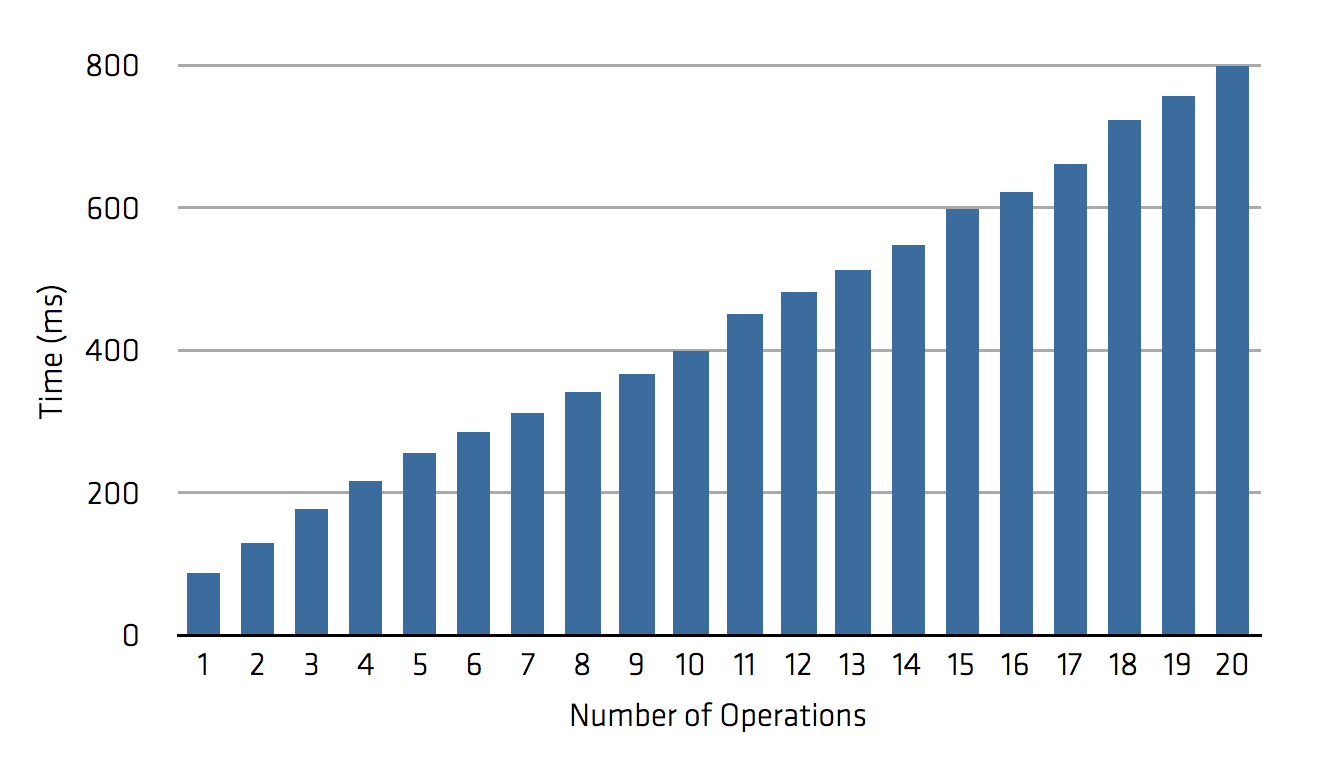
\includegraphics[width=0.9\linewidth]{time-long-final}
\caption{Running time in the Final Implementation}
\label{fig:runtimeFinal}
\end{figure}

\begin{figure}
\centering
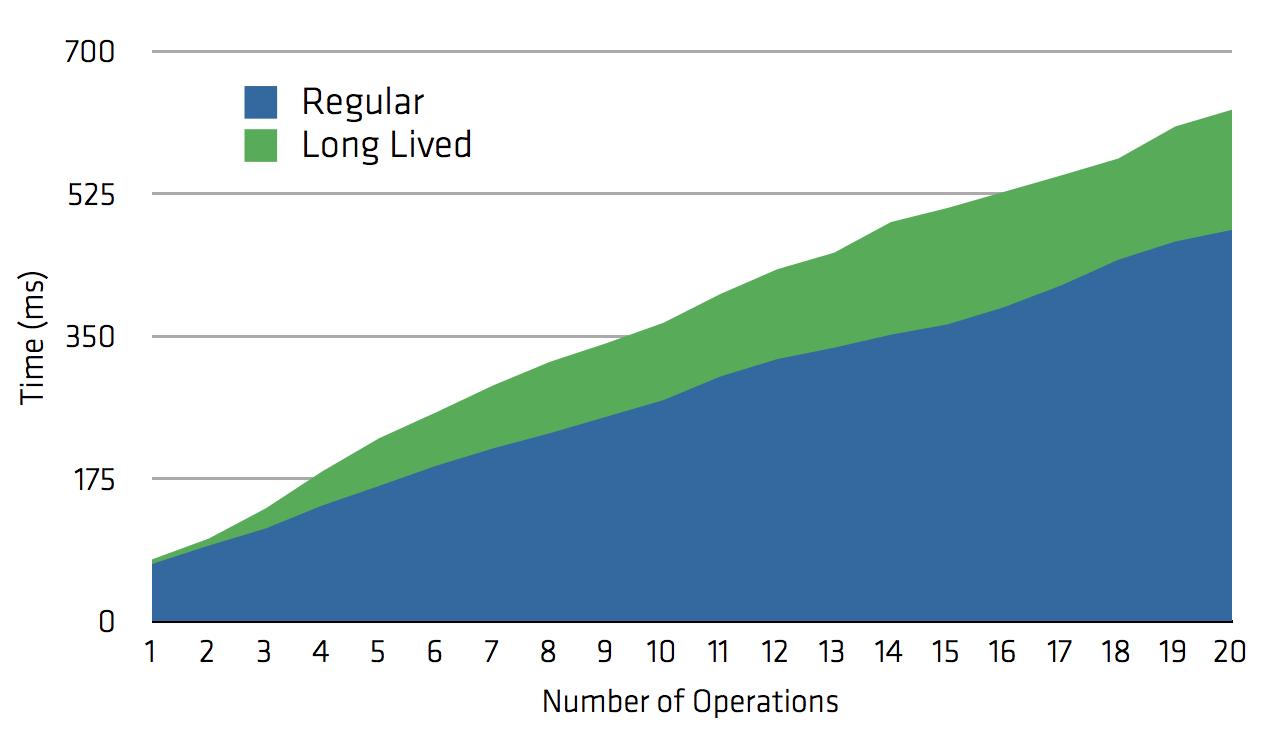
\includegraphics[width=0.9\linewidth]{comparison-final}
\caption{Running time comparison for the Final Implementation}
\label{fig:comparisonFinal}
\end{figure}


\begin{figure}
\centering
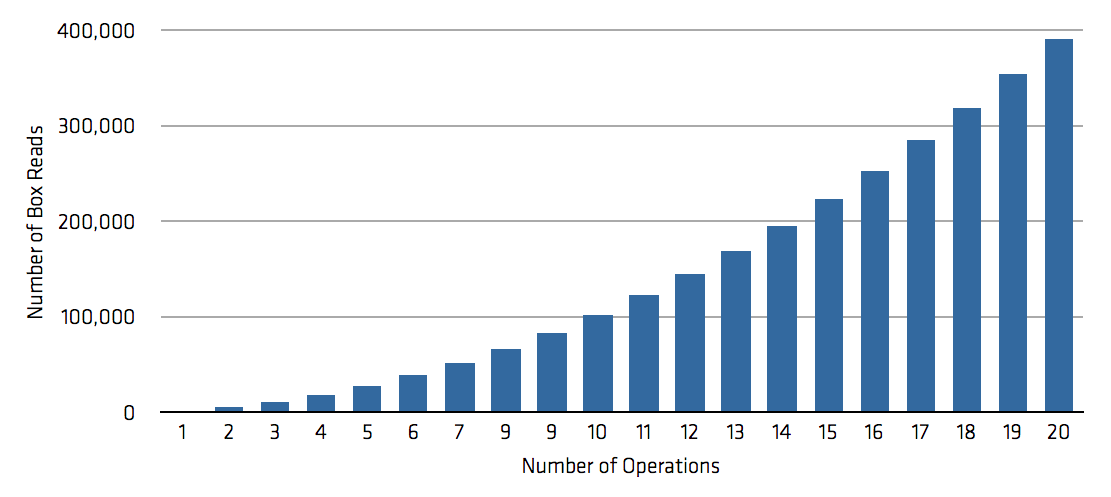
\includegraphics[width=0.9\linewidth]{box-long-final}
\caption{Box reads using Long Lived Transactions - Final Version}
\label{fig:boxesFinal}
\end{figure}

\begin{figure}
\centering
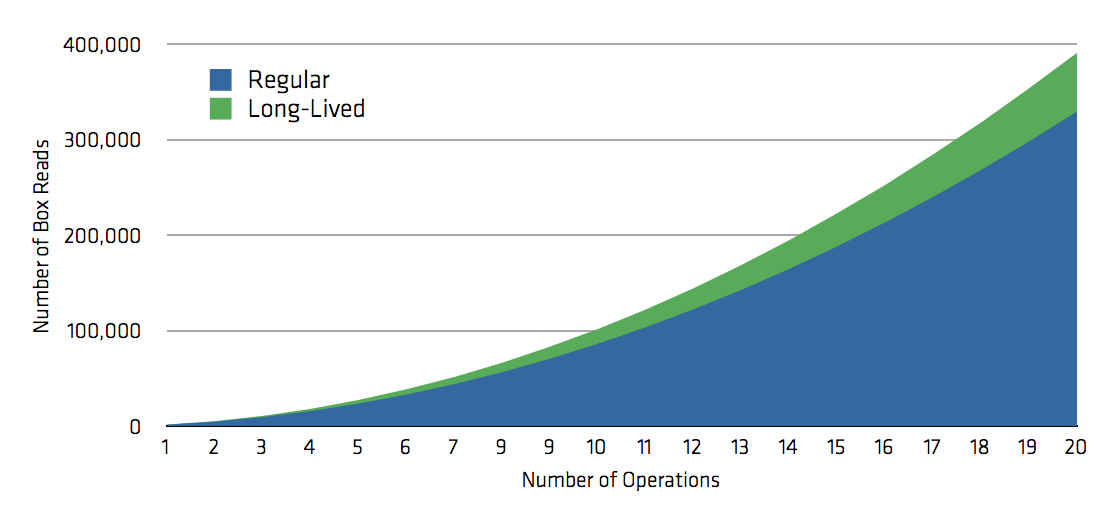
\includegraphics[width=0.9\linewidth]{box-comparison-final}
\caption{Box reads comparison for the Final Implementation}
\label{fig:boxComparisonFinal}
\end{figure}


